\section{Pattern recognition algorithms}
\label{cha:Introduction}
\subsection{Introduction}
Pattern recognition is a wide area of science in which we are interested in
assigning label from a given set of classes to every unknown pattern. The whole 
process of classification can be divided into few phases:
\begin{enumerate}
    \item Data collection
    \item Feature selection
    \item Model selection
    \item Classifier selection
    \item Training 
    \item Testing
\end{enumerate}
At first in this section few basic information and categories will be given 
about pattern recognition. Generally, the whole process of classification
can be broken down into two main categories
\begin{itemize}
    \item supervised - incoming to the system objects are not previously
        labeled and this is the system task to find an appropriate structure of
        the data, to establish the organization of the classes basing only on
        the available data, there is no statistical or expert knowledge at a
        hand.
    \item unsupervised - in this approach incoming patterns have labels and can
        be treated as a training set. This allows the classifier can retrieve
        information from data 
\end{itemize}
In this thesis supervised learning is reconsidered because available datasets 
are labeled with class number. When we take into account applied approach
pattern recognition, we can distinguish syntactic and statistical 
pattern recognition. In former each pattern is represented in terms of 
$d$ features, measurements and is viewed as a point in
$d$-dimensional feature space, while the latter
is  based on the characterization of the inherent structure of the 
qualitative features. For that  reason, the complex patterns can be
decomposed using a hierarchical structure in simple  sub-patterns.
The patterns are viewed as sentences belonging to a language, primitives
represents the alphabet of the language and the sentences are generated
according to a grammar which is inferred from the available training data.
EKG waveforms, textured images and shape analysis of contours are the examples
of syntactic approach.

\subsection{Problem statement}
\label{cha:Problem_statement}
In this section the problem statement will be presented in case of pattern
recognition. For the purpose of this thesis we assume supervised learning and
denote each pattern by the label $j \in M$, where $M$ is an $m$-element set of
possible states numbered with the successive natural numbers. The state $j$ is
unknown and does not undergo the direct investigation. What can only be
measured are attributes or features by which a state manifests itself. Each
object will be described by a $d$-dimensional measured feature vector $x \in
X$. In order to classify unknown pattern we use knowledge stored in training
set consisting of $N$ training patterns
$$S = (x_1, j_1), (x_2, j_2), \ldots, (x_N, j_N)$$
In practice the decision with learning should use knowledge included in the
training set $S$ and as the consequence the algorithm with learning is of the
following form:
$$i=\Psi(S, x), \, i \in M$$
In decision theory, to ensure that $\Psi$ approximate the problem as closely
as possible an additional loss function is introduced that assigns a specific
value to loss resulting from producing an incorrect label. The particular loss
function depends on the type of label being predicted. In case of
classification problem it is zero-one loss function. This corresponds simply to
assigning a loss of 1 to any incorrect labeling and is equivalent to computing
the accuracy of classification procedure over the set of training data.

\subsection{Rough sets}
\label{cha:Rough_set}
\subsubsection{Introduction}
\label{cha:Rough_set_introduction}
Rough sets theory represents mathematical approach to deal with imperfect knowledge. 
In the standard approach we need precise information about pattern to recognize, 
while rough sets can deal with vague or incomplete data. The problem of imperfect 
information was tackled for a long time and it became a crucial issue for many scientist.
One of the most prominent approaches in the recent years are fuzzy logic and rough sets.
In this section the latter approach is presented in greater details. Comparing with 
other methods rough sets have many advantages, but one of the most important
one is that it works only on the raw data, no additional information are needed such 
as density probability in Bayesian algorithm. The main facts about rough sets can be 
summarized in few point presented below:
\begin{enumerate}
    \item provides attribute reduction
    \item generates set of easy to understand and readable decision
        \textit{IF-THEN} rules
    \item evaluate significance of data 
\end{enumerate}

When talking about rough set theory one has to understand the concept of a set 
and how a rough set is related to the classical set represented in mathematic.
From the mathematical point of view the crisp (precise) set is a collection of 
objects of interest and is uniquely determined by its elements. In other words,
it means that every element must be uniquely classified as belonging to the set 
or not (true or false). For example, the set of odd numbers is crisp because every
number is either odd or even and cannot be partially in both. 

The nature of problem we met is much more complicated than simple decision that
objects belong to the set or not. For some sets we cannot precisely describe element
membership. Reconsider the group of people and division into set of small and
high people. The height is not a precise but a vague concept and data vagueness can 
be met in many problems found in the nature. Here is the spot for rough sets
theory where vagueness is expressed by a boundary region of a set. 

\subsubsection{Basic notation}
\label{cha:Rough_set_basic_notation}
In rough sets theory to represent datasets (information) we introduce a notion 
called an \textit{information system}. It can be described by 4-tuple
$$IS = <U, Q, V, f >$$ 
\begin{itemize}
    \item $U$ is the universe of discourse  which is a finite set of objects
    \item $Q$ is a finite set of attribute by  which each patterns manifests itself
    \item $V = \bigcup V_q$, $V_q$ represents a domain of attribute $q$
    \item $f:U \times Q \rightarrow V$ is a total information function, such that
        $\bigvee_{q\in Q, x \in U} f(x,q) \in U$
\end{itemize} 
The information system can be represented as a finite table in which 
columns are labeled by attributes and each rows stands for an object from
$IS$. Over the information table we can define decision table
$T$ where the set of attributes $Q$ is disjoined into two
subset $C$ and $D$. The set $C$ is a subset of 
condition attributes, and the set $D$ contains decision attributes 
by which we can partition set $U$ into decision classes.

From the granular nature of rough sets it may happen that some objects 
in the $U$ are indistinguishable due to the limited information. Now, let
define an indiscernibility relation $R \rightarrow U \times U$, representing the 
lack of knowledge about patterns in the set $U$. The indiscernibility relation on
$U$ can be extended and associated with every non-empty subset of attributes $P \subseteq Q$
and is defined as follows 
$$I_p = \{ (x, y) \in U \times U: f(x, q) = f(y,q), \bigvee_{q \in P}\}$$ 
Now having $I_p$ we can say that objects $x$ and
$y$ are $P$-indiscernible by a set of attributes $P$ is $y \, I_p \, x$. Relation
$I_p$ divides the set $U$ into blocks (concepts) of $P$-indiscernible objects.
The $P$-elementary set containing objects $P$-indiscernible with $x \in U$ is
referred as $I_p(x)$ and defined as follows:
$$I_p = \left\{ y \in U: y \, I_p \, x \right\}$$

By representing a target concept $X$ as a subset of $U$ we would like to
describe it with respect to $R$. Additionally let introduce $P$ as non-empty
subset of attributes from $Q$. In rough sets reasoning object membership to a
set can be represented in two ways:
\begin{enumerate}
    \item An object $x \in U$ certainly belongs to $X$ if
        all objects from the $P$-elementary set defined by $I_p(x)$ also belong to $X$.
        A set of all objects certainly belonging to $X$ creates the $P$-lower
        approximation of $X$ and can be represented as follows:
            $$\underline{I_p} = \{ x \in U: I_p(x) \subseteq X\}$$
    \item An object $x \in U$ can possibly belong to $X$ if at least one object
        from $P$-elementary set $I_p(x)$ can possibly belong to $X$. All the
        objects that could possibly belong to $X$ are denoted as $P$-upper
        approximation of $X$, defined as:
        $$\overline{I_p} = \{x\in U: I_p(x) \, \cap \, X \neq \emptyset \}$$
        Therefore the set $U - \overline{I_p}$ represents the negative region,
        containing the set of objects that can be definitely ruled out as
        members of the target set.
\end{enumerate}
The tuple $<\underline{I_p}, \overline{I_p}>$ representing a lower boundary of
the target $X$ and the upper boundary of the target $X$ creates a rough set.
Using above notions we can define $P$-boundary region which is a difference
between upper and lower approximation. 
$$BN_p(X) = \overline{I_p} - \underline{I_p}$$
The $BN_p(X)$ is a set of elements which cannot be certainly classified neither
as $X$ nor as not-$X$ with respect to the set of attributes $P$. If the
boundary region of $X$ is empty then it is crisp, otherwise we deal with
inexact set which is called rough set. Until that moment we can see that 
rough sets concept can be defined quite generally by means of topological
operations: interior and closure, called approximations. They express the
knowledge about pattern in terms of granules, not by a precise measure.

The illustrative example of rough sets reasoning is presented in fig.
\ref{fig:rough_set_example}
\begin{figure}[H]
    \begin{center}
        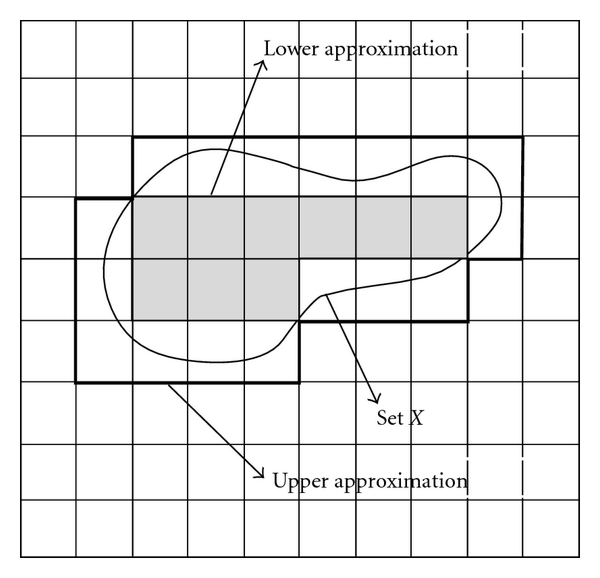
\includegraphics{fig/rough_set.png}
    \end{center}
    \caption{Rough sets example.}
    \label{fig:rough_set_example}
\end{figure}

\subsubsection{Rough sets indicators}
\label{cha:Rough_sets_indicators}
In rough sets theory we can define few indicators. First of all with every 
subset of $X \subseteq U$ described by $P$ subset of attributes we can 
associate an indicator called an accuracy of approximation defined as:
$$\alpha_p(X)=\frac{\underline{I_p}(X)}{\overline{I_p}(X)}$$

The quality of approximation of $X \subseteq U$ by attributes from subset $P$
represents the percentage of correctly classified objects using attributes $P$
from subset $X$
$$\gamma_P(X) = \frac{\overline{I_p}(X)}{|X|}$$
Assuming that we can partition $U$ into $n$ decision classes using $P$
non-empty subset of attributes from $C$, the quality of classification can be
defined as the ration of all correctly classified objects into classes
$$\gamma_P(CLASS) = \frac{\sum_{i=1}^{n}\overline{I_p}(CL_i)}{|U|}$$
These indicators can be used in determining the quality of rough set algorithm
or for finding the optimal reduct.
\subsubsection{Properties of rough sets}
The same as classical sets or fuzzy logic rough sets can be described by the
following properties:
\begin{enumerate}
    \item $\overline{I_p} \subseteq \, X \, \subseteq \, \underline{I_p}$
    \item $\overline{I_p}(\emptyset) = \underline{I_p}(\emptyset) = \emptyset;
        \;
        \overline{I_p}(U) = \underline{I_p}(U) = U $
    \item $\overline{I_p}(X \cup Y) = \overline{I_p}(X) \cup \overline{I_p}(Y)$
    \item $\underline{I_p}(X \cap Y) = \underline{I_p}(X) \cap \underline{I_p}(Y)$
\end{enumerate}
% TODO Dokonczyc to

\subsubsection{Attribute reduction}
\label{cha:Rough_set_attribute_reduction}
Many problem are complex and multidimensional. For example Sonar dataset from
\textit{UCI} Repository has 60 attributes describing a single pattern. 
Usually we hope to recognize pattern in a relatively
lower dimensional to reduce cost in measuring and processing information and
enhance the interpretability of learned models. Feature selection or reduction 
is done for classifiers to remove the noise and superfluous data. Generally,
this is not an easy task and requires a lot of computation. 


A reduct is a set of attributes that ensures the same classification of
elements from $U$ as the rudimentary set of attributes. More than one reduct
can exist for one information system. The core of attributes is the set of
attributes from $Q$ that all the attributes are indispensable. An attribute is
dispensable if the following criterion is fulfilled:
$$I(P) = I(P-{a}), \, \textrm{for} \, \{a\} \in P \subseteq  Q $$

\subsubsection{Rough sets reasoning from data}
The category description can be done in two ways:
\begin{enumerate}
    \item extensional
    \item intentional
\end{enumerate}
To represent a concept we have to be able to identify all objects belonging 
to this category. With the former approach we have no insight 
into decision engine so we do not know how to assign new objects to the category.
In the latter approach we represent the category based on the set of rules. The same 
approach is done in rough sets algorithm where an elementary 
granules (concepts) of knowledge build blocks consisting 
of indiscernible pattern from the universe of discourse. 
We will associate decision rules with decision table $T$.

In this section a practical example will be presented to clear all the things
out. As an example let reconsider well-known example of patients suffering from
flu. 
\begin{table}[H]
    \centering
    \caption{Example dataset showing healthy patients and suffering from flu}
    \begin{tabular}{|c|c|c|c|c|c|}
        \hline 
    Patient & Headache & Muscle pain & Temperature & Flu \\ \hline \hline
    p1 & no & yes & high & yes \\ \hline
    p2 & yes & no & high & yes \\ \hline
    p3 & yes & yes & very high & yes \\ \hline
    p4 & no & yes & normal & no \\ \hline
    p5 & yes & no & high & no \\ \hline
    p6 & no & yes & very high & yes \\ \hline    
    \end{tabular}
    \label{tab:example_rough_set}
\end{table}
Table \ref{tab:example_rough_set} represents an information system about
healthy patient and those suffering from flu. Attributes: Headache,
Muscle-pain, Temperature are called condition attributes, while the attribute
``Flu'' (last column in table \ref{tab:example_rough_set}) is considered as
decision attribute. Each row of a decision table determines a decision rule,
for example

IF HEADACHE IS 'NO' AND MUSCLE\_PAIN IS 'YES' AND TEMPERATURE IS 'HIGH' THEN FLU IS 'YES'

Here we can generate few indiscernible relations based on 
the chosen attributes. In case of Headache attribute patients p2, p3, p5 are indiscernible; patients p2, p5 are
indiscernible with respect to attributes Headache, Muscle-pain and Temperature. 
Using Headache and Muscle-Pain we can divide the set into three sets:
\{p1, p4, p6\}, \{p2, p5\}, \{p3\}.

Now it is time for defining key features of rough sets. Over the table
\ref{tab:example_rough_set} we can define two concepts: ``Flu'' and
``Not Flu''. For the first concept the lower approximation
set of patient certainly having flu is \{p1, p3, p6\}, while the upper
approximation of patients possibly suffering from flu is \{p1, p2, p3, p5,
p6\}. The boundary region for concept ``flu'' is a set of \{p2, p5\} patients. 
For the concept ``Not Flu'' the lower approximation is the set \{p4\}, whereas
the upper approximation is the set \{p2, p4, p5\}. Again the boundary region is
the set \{p2, p5\}.

Additionally, we can measure the accuracy of approximation $\alpha_P(x)$ for each concept.
This can tell us if the set of attributes to describe the concept is correctly
chosen. For the ``Flu'' concept where $X$=\{p1, p2, p3, p6\} is described by
set of attributes $P$=\{Headache, Muscle-pain, Temperature\} the accuracy of
approximation is $\alpha_P(Flu) = \frac{3}{5}$. On the other hand when we take
only one attribute $P$=\{Temperature\}, then we get lower approximation of \{p3,
p6\} and upper approximation of \{p1, p2, p3, p5, p6 \} resulting in
$\alpha_P(Flu) = \frac{2}{5}$. To sum up, $\alpha_P(x)$ is a very important indicator in
rough sets theory and tells which attributes better characterize target
concept. 


\subsection{Fuzzy logic}
\label{cha:Fuzzy_logic}
\subsubsection{Introduction}
In fuzzy logic an element membership to a set is described by membership function 
which assigns value from interval $<0, 1>$. It is a superset of Boolean logic that 
has been extended to handle the concept of partial truth - values between ``completely 
true'' and ``completely false''. It was introduced by Dr. Lotfi Zadeh in the
1960's as a tool to model the uncertainty of natural language. As in the
section \ref{cha:Rough_set_introduction}, let introduce the problem of defining 
if person is small or high. 

First of all, we have to define a fuzzy set \textit{TALL} which will answer the question 
"to what degree is person x tall?". Zadeh describes \textit{TALL} as a LINGUISTIC VARIABLE, 
which represents our cognitive category of "tallness". To each person in the universe of discourse, 
we have to assign a degree of membership in the fuzzy subset \textit{TALL}. The easiest way to do this
is with a membership function based on the person's height. Given this definition, here are some example values
\begin{table}[H]
    \centering
    \caption{Table describing how person is tall by the fuzzy logic linguistic
    variable}
    \begin{tabular}{|c|c|c|}
        \hline
        Person & Height [m] & degree of tallness \\ \hline \hline
        p1 & 1.5 & 0.0 \\ \hline
        p2 & 1.6 & 0.2 \\ \hline
        p3 & 1.7 & 0.4 \\ \hline
        p4 & 1.8 & 0.5 \\ \hline
        p5 & 1.9 & 0.6 \\ \hline
        p6 & 2.0 & 1.0 \\ \hline
    \end{tabular}
    \label{tab:fuzzy_logic_example}
\end{table}

Fuzzy numbers are fuzzy subsets generated over the attribute domain. 
They have a peak or plateau with membership grade 1, over which the 
members of the universe are completely in the set.  The membership 
function is increasing towards the peak and decreasing away from it. 
There are different types of membership functions and their usage 
strongly depends on the type of reconsidered problem. One of the most 
common met in the literature are: triangular, trapezoidal, Gaussian shapes
(see example on ).

\subsubsection{Fuzzy reasoning from data}
Reasoning in fuzzy logic is based on decision rules the same as in rough sets approach. 
Rules are expressed in the form of IF \textit{COND} THEN \textit{DECISION} 
which can be divided into antecedent set and one consequent. 
The \textit{AND}, \textit{OR}, and \textit{NOT} operators of 
Boolean logic exist in fuzzy logic, usually defined as the minimum, maximum,
and complement. When they are defined this way, they are called the Zadeh operators.
Fuzzy logic classification is based  on three steps:
\begin{enumerate}
    \item Fuzzyfication- in the fuzzyfication process we 
        convert continuous quantity into fuzzy number. It requires defining
        membership grade of crisp input $x$ in the fuzzy set.
    \item Rule induction- there are different types of fuzzy inference systems,
        but one of the most commonly used (the same as in this paper) is
        Mandami inference system.
    \item Deffuzification- the process of producing a quantifiable result in fuzzy logic,
        given fuzzy sets and corresponding membership degrees. These will have a number of
        rules that transform a number of variables into a fuzzy result, that is, the result 
         is described in terms of membership in fuzzy sets. 
\end{enumerate}
Let reconsider a simple example, which should clear all ambiguities (the following 
example is based on \cite{bib20}). The problem is connected with estimating the
level of risk involved in software engineering project. There are two input
to the system (funding, staffing) and one output
(risk). Membership functions are represented as triangular shapes (fig. \ref{fig:fuzzy_example_1}) 
\begin{figure}[H]
    \begin{center}
        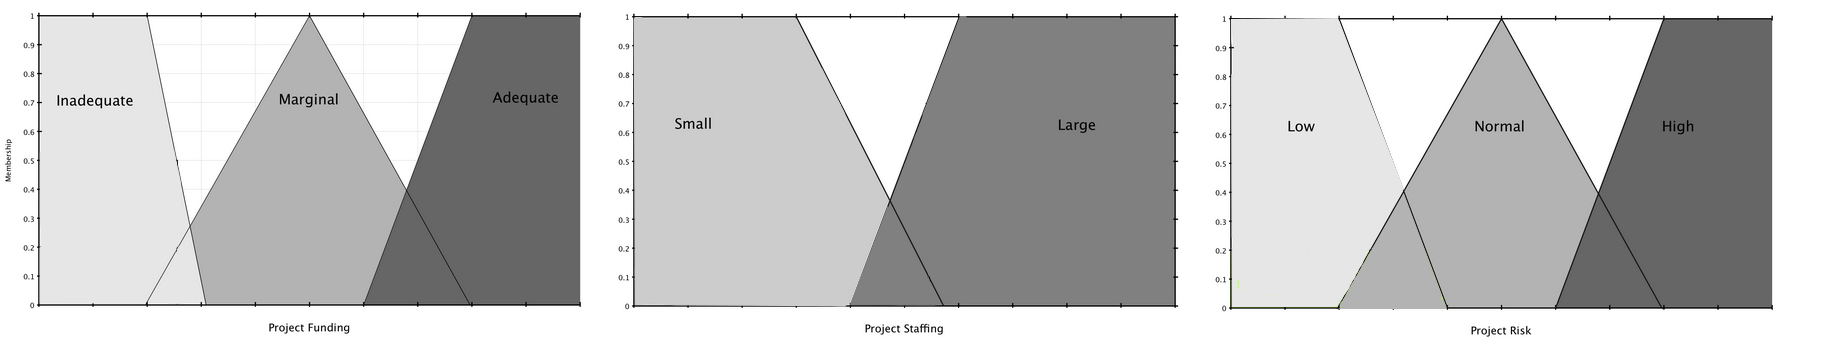
\includegraphics[width=\textwidth]{fig/fuzzy_example_1.png}
    \end{center}
    \caption{Input and output fuzzy linguistic variables for the described
    system.}
    \label{fig:fuzzy_example_1}
\end{figure}
The next important thing in fuzzy logic beside fuzzy values are fuzzy rules. In
this problem they are provide a priori and are in the following way:
\begin{table}[H]
    Rule 1: IF funding IS adequate OR funding IS small THEN risk IS
    low \\
    Rule 2: IF funding IS marginal AND staffing IS large THEN risk IS
    normal \\
    Rule 3: IF funding IS inadequate THEN risk IS high
\end{table}
Let say we want to calculate project risk for inputs funding~$=35$ and
staffing~$=60$. 
\begin{enumerate}
    \item The first step is to convert crisp values into fuzzy representation.
        $$
            \begin{array}[H]{l}
                \hline
                \mu_{inadequate}(35) = 0.5 \\
                \mu_{marginal}(35) = 0.2 \\
                \mu_{adequate}(35) = 0.0 \\ \hline
                \mu_{small}(60) = 0.1 \\
                \mu_{large}(60) = 0.7 \\ \hline
            \end{array}
        $$
    \item Now it is time for rule induction where OR is treated as a $max$ operator, AND
        as $min$ operator. 
        $$
            \begin{array}[H]{ll}
                Rule \,1: & \mu_{low} = 0.0 + 0.1 = 0.1 \\
                Rule \,2: & \mu_{normal} = 0.2\cdot 0.7 = 0.14 \\
                Rule \,3: & \mu_{high} = 0.5 \\
            \end{array}
        $$
    \item After performing clipping of consequent membership functions for each
        rule (example given in fig. \ref{fig:fuzzy_centroid}), the final crisp output can be calculated. It is done by
        defuzzification method, where one of the most commonly used is a centroid
        formula given by eq. (\ref{eq:fuzzy_centroid})
        \begin{equation}
            CO = \frac{\sum\nolimits_{x=a}^{b}\mu_A(\chi)\cdot
            x}{\sum\nolimit_{x=a}^{b}\mu_A(\chi)}
            \label{eq:fuzzy_centroid}
        \end{equation}
        \begin{figure}[H]
            \begin{center}
                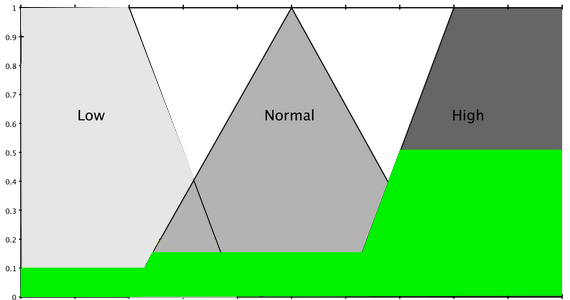
\includegraphics[width=0.8\textwidth, height=0.5\textwidth]{fig/fuzzy_centroid.png}
            \end{center}
            \caption{Example of clipping the consequent membership function
            as the result of rule induction}
            \label{fig:fuzzy_centroid}
        \end{figure}
        Using eq. (\ref{eq:fuzzy_centroid}) the output of the system is as follows:
        $$
        CO = \frac{(0+10+20)\cdot 0.1 + (30+40+50+60)\cdot 0.14 + (70 + 80 + 90
        + 100)\cdot 0.5}{0.1\cdot 3 + 0.14\cdot 4 + 0.5\cdot 4 } = 69.3
        $$

\end{enumerate}
\subsubsection{Genetic-based machine learning approaches}
In the literature one can find many examples of fuzzy logic applications.
Generally, there are two main approaches:
\begin{enumerate}
    \item some expert knowledge is available and fuzzy rules are created
        beforehand.
    \item no knowledge about data set is available so some techniques of data
        mining must be applied to extract rules from training set.
\end{enumerate}
At this point it must be strongly emphasize that the main focus is based on
fuzzy algorithm for pattern recognition task where there is no prior knowledge 
about fuzzy system. There are different approached from optimization techniques
such as gradient descent to heuristic. In this thesis the genetic algorithm
will be used. 

If until this point something is unclear reconsider the following example. What
we have is the problem dimensionality and the set of training patterns. Now the
questions arise such as: how to divide feature space into fuzzy set, how
generate rule. For example, we create 10 triangular membership functions for each
attribute, but is this number optimal. Secondly, when we have $d$-dimensional
feature space and $k$ fuzzy membership function per each attribute
the number of possible combination for generating one rule is equal to $k^d$.
For greater $d$ (for example Sonar dataset from \textit{UCI} repository has 60
attributes) it is impossible to find the proper combination in a reasonable
time.

There are two main methods of genetic-based machine learning approaches:
\begin{enumerate}
    \item Michigan template- it is a population of fuzzy rules and a single
        fuzzy rule is handled as an individual. The evaluation of each fuzzy
        rule is performed by classifying all the given training patterns by the
        available rule set $N_{rule}$. At the end of each iteration new
        individuals are created through genetic operators and merged to the
        current population. For the next generation $N_{rule}$ best individuals
        are taken. The whole procedure can be summarized as follows:
        \begin{enumerate}
            \item Generate $N_{rule}$ fuzzy rules
            \item Evaluate the fitness of each fuzzy rule in the current
                population
            \item Generate $N_{replace}$ fuzzy rules using genetic operators
            \item Merge $N_{replace}$ fuzzy rules with current population and
                choose the best $N_{rule}$ individuals for the next generation
            \item Return to point $(b)$ is stopping condition is not fulfilled
        \end{enumerate}
    \item Pittsburgh template- in this approach a set of fuzzy rules is handled
        as an individual. In this case the length of a single individual is
        equal to $n\cdot N_{rule}$, where $n$ is the length of a fuzzy rule.
        Algorithm starts with $N_{pop}$ randomly generated rule sets. The
        fitness value of a single individual is the number of correctly
        classified patterns in the training set by a given rule set.
        The procedure for algorithm is as follows:
        \begin{enumerate}
            \item Generate $N_{pop}$ individuals consisting of $N_{rule}$ fuzzy
                rules each
            \item Calculate the fitness value of each rule set (individual)
            \item Generate $N_{replace}$ new rule set using genetic operators.  
            \item Merge $N_{replace}$ fuzzy rule sets  with current population and
                choose the best $N_{pop}$ individuals for the next generation
            \item Return to point $(b)$ is stopping condition is not fulfilled
        \end{enumerate}
\end{enumerate}
\subsection{Genetic algorithm}
\label{cha:Genetic_algorithm}
Genetic Algorithm is an element of evolutionary computation, which is a 
rapidly growing area of soft computing. GA is based on the principles of
natural selection and genetic modification. As optimization methods, GA 
operates on a population of points, designated as individuals. Each 
individual of the population represents a possible solution of the 
optimization problem. Individuals are evaluated depending upon their 
fitness which indicates how well an individual of the population solves 
the optimization problem. To sum up, GA has the following general features:
\begin{enumerate}
    \item GA operates with a population of possible solutions (individuals) 
        instead of a single individual. Thus, the searching process can be 
        carried out in a parallel form or sequentially.
    \item GA is able to find the optimal or sub-optimal solutions in complex
        and large search spaces. Moreover, it can be applied to nonlinear 
        optimization problems with constraints defined in discrete or continuous 
        search spaces.
    \item GA examines many possible solutions at the same time, so there is a 
        higher probability that the search process can converge to an optimal solution.
\end{enumerate}
There are four main parts in each GA process to reconsider:
\begin{enumerate}
    \item the problem representation or encoding
    \item fitness or objective function definition
    \item fitness-based selection
    \item evolutionary reproduction of candidate solutions (individuals or chromosomes). 
\end{enumerate}
Genetic algorithms are widely used as a search techniques in the various fields. 
In this thesis it will be used for finding optimal cuts in the attribute space and to 
apply attribute reduction. The success of a genetic algorithm can be quantified by estimating 
the cost, time required and the quality of final obtained solution. 
In the literature there can be found many examples of how GA is useful in solving hard 
optimizations problems, but beside unquestionable advantages there also exist downsides. 
A traditional GA without any diversity maintenance mechanism often suffers from getting 
stuck on the suboptimal peaks, because almost the entire GA population would have converged 
to a single peak, as a result of the rapid loss of population diversity. 
There is a great deal of work showing how to set the optimal parameters in an evolutionary 
algorithm to obtain required speedup and solution accuracy, but this is not the main issue 
in this thesis. For more exact information see .
When designing genetic algorithm one of the most important things to ensure proper crossover 
and mutation operations. More precise information about these operation will be
presented in section \ref{cha:Algorithm_construction_genetic}

\subsection{Hybrid classifiers}
\label{cha:Hybrid_classifiers}
In the recent years, there is an increasing interest in methods of combining
multiple learning systems into hybrid one. The main advantage of such approach
is its ability to find different explanation for the dataset for each
classifier. If classifiers make errors on different parts of the feature space
it is possible that the ensemble of classifiers will complement each other and
the final classification will be better. 

Generally, there are two types of hybrid classifiers (example presented in fig.
\ref{fig:hybrid}:
\begin{enumerate}
    \item multiexpert systems- classifiers work in parallel, each of them is
        trained and tested on the same data and independent decisions are
        combined to compute the final result. The most common example is a
        majority voting 
    \item multistage systems- classifiers are connected in a sequence where the
        next classifier is trained and used for classification only if the
        previous classifier rejected the pattern. 
\end{enumerate}
It is hard to determine which approach is the best. Each system has its pros
and cons and the choice depends of the type of dataset. In this thesis the second 
approach is implemented.
\begin{figure}[H]
    \begin{center}
        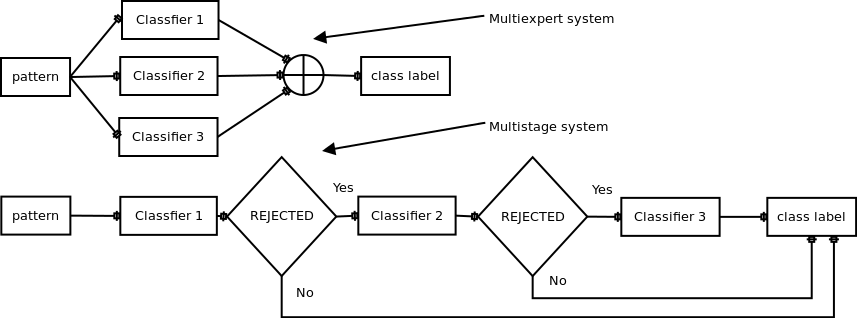
\includegraphics[width=\textwidth]{fig/hybrid.png}
    \end{center}
    \caption{Example of two approaches for constructing hybrid classifiers}
    \label{fig:hybrid}
\end{figure}

